\section{Evaluation of the Project}
Testing and evaluation were vital parts of the project, to ensure that the system produced, both contained all the functionality it should have, it adhered to all the constraints place upon it and that it was actually usable. Three stages of testing were therefore conducted. The first of these was functionality testing, in which the functional requirements of the system would be evaluated, and the system would be testing to see whether or not it implements this functionality. The next stage was non-functional testing, in which the non-functional requirements would be evaluated in turn, to ensure the system abided by them. The final stage was user feedback testing, in which a group of participants would actually be using the system. In this stage, three systems would be evaluated: MATLAB, FuzzyToolkitUoN, and this project; in order to determine which provided a better user experience.

\subsection{Functional Testing}
In this section, each of the functional requirements laid out in section \ref{sec:funcs} have been evaluated in turn, to ensure the system meets them. Knowledge of the inner workings of the system is not actually necessary to understand these tests, as they simply check whether functionality is present, and are not concerned as to how the system actually implements it (this is known as black box testing \cite{beizer1995black}). A complete listing of all the tests conducted, and their results, can be found in appendix \ref{app-ctl}.

\subsection{Non-Functional Testing}

\subsection{User Feedback Testing}
\label{sec:uft}

% mention how someone obviously said the errors were friendly

% as part of jakon nielsons usability engineering life cycle 
\cite{nielsen1992usability}
% i did some user evaluation%%%%%%%%%

%	{\color{red}
%		Comparisons against other software, and checking against non-functional requirements. General explanation about the tests, and the participants, and what we are looking for (non functional, usability, accessibility). talk about using disseration to do fuz coursework. ``Considering I wrote both FTU and oFuzz, i found oFuzz much easier to use. Having the fuz coursework gave me a unique experience to test using both systems, as a user, instead of as the developer.''
		
%		{\color{blue}
%		An important part of evaluating the usability and accessibility of my system was to have real world users attempt to actual use not only my system, but similar systems, so that they could make comparative comments. In order to do this, I set up several sessions in which I would invite users of various skills levels, both in terms of computers, and fuzzy logic, to complete a list of tasks using all three software systems, after which I would ask them to give their feedback and opinions on all the systems. The three software systems that were evaluated were: my project, the MATLAB fuzzy toolbox, and FuzzyToolkitUoN, within the standard R environment.\ \\
%		\ \\
%		I split the participants into four main categories, based on their skill levels in terms of using computers, and knowledge of fuzzy logic. There were a total of 23 participants in these studies, and the distribution of skill levels is displayed in figure \ref{fig-skills}. The reason for this split was so that these distinctive groups could be evaluated individually, and their specific requirements could be observed. For instance, a participant skilled in computers, but not in fuzzy logic, would not struggle in navigating a system, but could potentially struggle understanding some of the fuzzy terminology.
		
%		\begin{figure}[ht!]
%		\begin{center}
%		\begin{tabular}{cc|cc}
%			& &\multicolumn{2}{c}{Computer Skill} \\
%			& & Low & High \\
%			\hline 
%		    \multirow{2}{2cm}{Fuzzy Logic Skill}  & Low & 7 & 5  \\
%		     &  High                                    & 3 & 8  \\
%		     \hline
%		     \\
%		     \multicolumn{3}{r}{\textbf{Total}} & 23\\
%		\end{tabular}
%		\end{center}
%		\vspace{-5mm}
%		\caption{Distribution of participant skill levels}
%		\label{fig-skills}
%		\vspace{-2mm}
%		\end{figure}
%		\noindent 
%		The task assigned to the participants was designed to use as much of the different systems as possible, but focused mainly on cross-compatible parts of the systems, so they could be easily compared. The test itself was to construct the fuzzy tipper example, using service and food as inputs, to produce a number for the tip to leave (the full set of instructions can be found in appendix \ref{app-userEval}). 
%		}
%	}
	\subsubsection{Evaluation of FuzzyToolkitUoN}
%		{\color{red}
%			Good things, bad things, statistics to back this up, talk about non funcs, and mention each type of user
%		}
	\subsubsection{Evaluation of MATLAB Fuzzy Toolbox} 	
%		{\color{red}
%			As above, but comparisons with above. specificaly mention that MATLAB has milliions of windows to open which make it very confusing!!!		
%		}
	\subsubsection{Evaluation of My Project}	
%		{\color{red}
%			As above, but comparison with above and above above
%		}
	\subsubsection{Summary}	
%		{\color{red}
%			Overall results and comparative statistics. 
%			{\color{blue}
%			The main two factors that were observed whilst the participants were completing the tasks were the speed at which they could do so, and the ease. Generally a faster completion meant either a high level of understanding, or an easier piece of software to use. The data collected strongly suggests that completion of the task using FuzzyToolkitUoN was the most difficult, which after speaking to the participants was the result of a poor user interface, and a very steep learning curve (especially for those of a novice computer skill level). The graph in figure \ref{fig:times} shows box plots of the completion times of each of the tasks, for each of the different groups. Each of these plots shows that FuzzyToolkitUoN was the most time consuming task to complete (taking on average {\color{red} 100 seconds}), and that the graphical systems were much easier to use (with MATLAB on average, taking {\color{red} 40 \%} less time, and my new system taking {\color{red} 10 \%} less time than that).
			
%			\begin{figure}[ht!]
%			\begin{center}
%			some graph yo
%			\end{center}
%			\vspace{-5mm}
%			\caption{Time taken to complete the tasks in the different software systems}
%			\label{fig:times}
%			\vspace{-2mm}
%			\end{figure}
			
%			Whilst the time taken to complete the tasks was a strong indicator of the success of the software system, it was also important to ask the participants which system they enjoyed using the most. The results for this were conclusive, which 100\% of participants (across all categories) claiming FuzzyToolkitUoN was the piece of software they enjoyed using the least. {\color{red} This is because...}. The piece of software that the participants enjoyed using the most was {\color{red} x \%} in favour of my produced software, over MATLAB (and the majority of those that said they preferred MATLAB said so as they were already very familiar with MATLAB). The results for most favoured,  software system can be seen in figure \ref{fig:mostleast}, organised by category of participant. {\color{red} The main reasons for an attraction to MATLAB were... and o-fuzz}
			
%			\begin{figure}[ht!]
%			\begin{center}
%			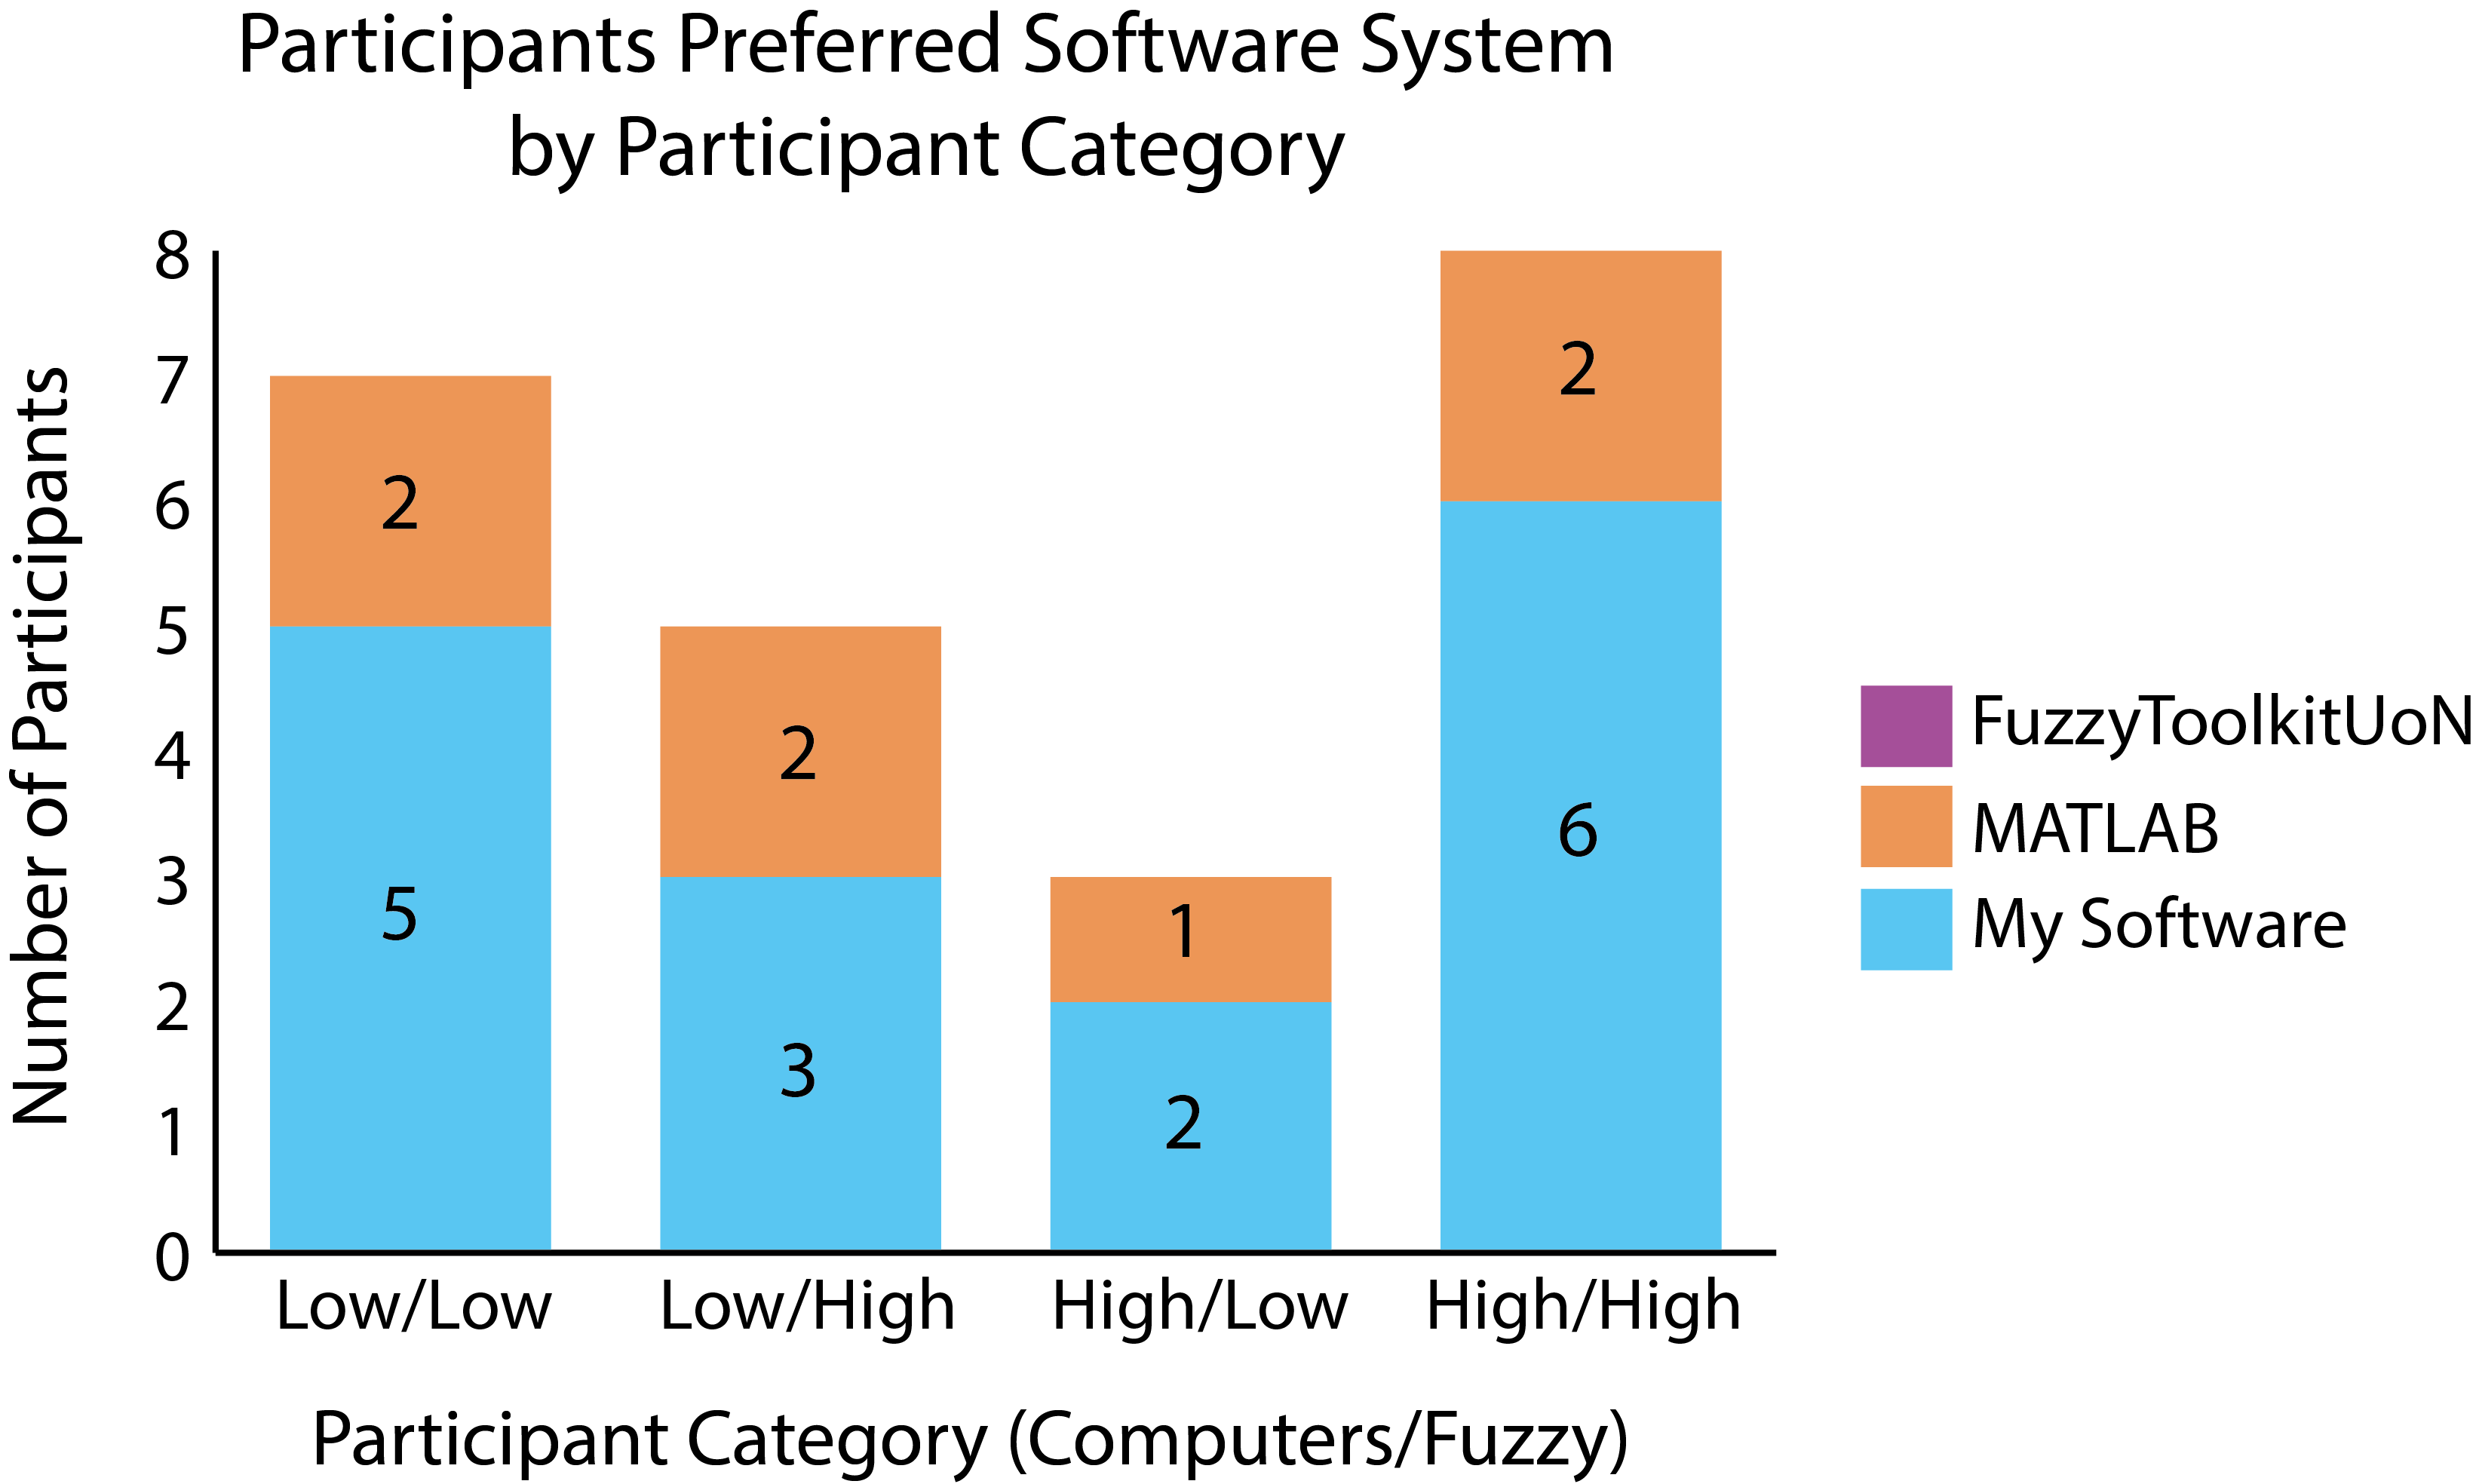
\includegraphics[width=0.8\textwidth]{images/graphsSmall.png}
%			\end{center}
%			\vspace{-5mm}
%			\caption{Favoured/Least Favoured software system, by participant category}
%			\label{fig:mostleast}
%			\vspace{-2mm}
%			\end{figure}
%			}
%		}		

\subsection{Successes and Limitations of the Project}
%{\color{red} 
%Explain what went well with the project, what didn't go so well, and what could be done better for next time (with concrete goals). issues with FTU as the backend (some options in params disabled because they don't work in FTU - not my fault!).

%}